\documentclass[a4paper,onecolumn]{extarticle}
\usepackage{geometry}
\usepackage[page,toc,titletoc,title]{appendix}
\usepackage{url}
\usepackage{caption}
\usepackage{subfigure}
\usepackage{subcaption}
\usepackage[sc]{mathpazo} % Use the Palatino font
\usepackage[T1]{fontenc} % Use 8-bit encoding that has 256 glyphs
\usepackage[utf8]{inputenc} % Use utf-8 as encoding
\linespread{1.05} % Line spacing - Palatino needs more space between lines
\usepackage{microtype} % Slightly tweak font spacing for aesthetics
\usepackage[spanish, activeacute]{babel}
 \decimalpoint
% \usepackage[hmarginratio=1:1,top=32mm,columnsep=20pt]{geometry} % Document marginshttps://www.overleaf.com/project/60211b96f72a79d4c7515e93
% \usepackage[hang, small,labelfont=bf,up,textfont=it,up]{caption} % Custom captions under/above floats in tables or figures
\usepackage{verbatim} % comentarios
\usepackage{listings}
\usepackage{xcolor}
\usepackage{wrapfig}
\lstset{
    inputencoding=utf8,
    frame=single,
    basicstyle=\fontsize{7}{10}\selectfont\ttfamily,
    basicstyle=\ttfamily\small,
    keywordstyle=\color{blue}\bfseries,
    identifierstyle=\color{black},
    commentstyle=\color{gray}\itshape,
    stringstyle=\color{red},
    numbers=left,
    numberstyle=\tiny\color{gray},
    stepnumber=1,
    numbersep=10pt,
    showspaces=false,
    showstringspaces=false,
    breaklines=true,
    breakindent=0pt,
    breakatwhitespace=false,
    tabsize=2,
    captionpos=b,
    literate={á}{{\'a}}1
        {ã}{{\~a}}1
        {é}{{\'e}}1
        {ó}{{\'o}}1
        {í}{{\'i}}1
        {ñ}{{\~n}}1
        {¡}{{!`}}1
        {¿}{{?`}}1
        {ú}{{\'u}}1
        {Í}{{\'I}}1
        {Ó}{{\'O}}1
}
\setlength{\parskip}{0.8em}
\usepackage{natbib}
\usepackage{enumitem}
% \setlist[itemize]{noitemsep} % Make itemize lists more compact
% \usepackage{abstract} % Allows abstract customization
% \renewcommand{\abstractnamefont}{\normalfont\bfseries} % Set the "Abstract" text to bold
% \renewcommand{\abstracttextfont}{\normalfont\small\itshape} % Set the abstract itself to small italic text
\usepackage{titlesec}

\usepackage{fancyhdr} % Headers and footers
\pagestyle{fancy} % All pages have headers and footers
\fancyhead{}
\lhead{Hugo Gómez Sabucedo}
\rhead{Minería de datos y modelización predictiva}

\renewcommand{\footrulewidth}{0.2pt}
\usepackage{titling} % Customizing the title section
\usepackage[breaklinks=true]{hyperref} % For hyperlinks in the PDF
%\usepackage{array}
%\newcolumntype{C}[1]{>{\centering\let\newline\\\arraybackslash\hspace{0pt}}m{#1}}
\usepackage{graphicx}
%\usepackage{lipsum} % NO NECESARIO LUEGO
%\usepackage{amsmath}
%\usepackage{wrapfig}
%\usepackage{multicol}
%\usepackage{bm}


\let\stdsection\section
\renewcommand\section{\newpage\stdsection}

%-------------------------------------------------------------------------------
%	TITLE SECTION
%-------------------------------------------------------------------------------

\setlength{\droptitle}{-4\baselineskip} % Move the title up



\title{\begin{center} \Huge Minería de datos y modelización predictiva: Series Temporales\end{center}} % Article title
\author{
    \textsc{\Huge Hugo Gómez Sabucedo} \\ % Your name
    \large \href{mailto:hugogomezsabucedo@gmail.com}{hugogomezsabucedo@gmail.com} \\ [2ex] % Your email address
    \Large \textbf{Máster Big Data, Data Science \& Inteligencia Artificial} \\
    \normalsize Curso 2024-2025 \\
    \large Universidad Complutense de Madrid
}
\date{} % Leave empty to omit a date

\begin{document}
% Print the title
\maketitle
%\newpage
\tableofcontents
%\newpage
\begin{sloppypar}

%-------------------------------------------------------------------------
%	DOCUMENT
%-------------------------------------------------------------------------

\section{Introducción y análisis inicial} \label{introduccion}
\subsection{Introducción} \label{intro}
En este ejercicio se realizará el análisis y predicciones sobre una serie temporal, con datos obtenidos a partir del Instituto Nacional de Estadística. Estos 
datos, disponibles en el archivo \texttt{viajerosMD.xlsx}, que contienen los datos sobre los viajeros totales en ferrocarril de media distancia en España, 
medidos en \textbf{miles de viajeros}, desde el año 2010 hasta el 2024, medidos mensualmente. Aunque la serie original contiene datos que se remontan al año 2000, 
para no tener una serie tan grande, se ha decidido elegir únicamente estos datos. Por lo tanto, la serie constará de 15 años, o lo que es lo mismo, 180 
observaciones, de las cuales, en lo que se corresponde al punto 3 del enunciado de la práctica, reservaremos 12 para realizar el test de los modelos, siendo 
las 168 restantes los datos con los que entrenaremos el modelo.

El código completo de Python de esta práctica se adjunta en el archivo \texttt{codigoMineria3.py}, también al final de este documento, por lo que aquí sólo 
incluiremos \textit{snippets} de código que sean especialmente relevantes o que no se hayan visto en clase. Antes de comenzar con el análisis, debemos 
naturalmente importar el archivo en Python, y realizar una serie de pequeñas modificaciones. Estas consisten en transformar la fecha, para que sea un formato 
de fecha legible por Python. En el archivo original el formato es \textit{    2024M12}, por lo que empleamos el siguiente código para realizar la conversión 
(líneas 1 y 2). Además, transformamos los datos de la serie, los valores numéricos, para que se consideren como un número y no como string (línea 3), y se 
establece la fecha como índice (línea 4). Por último, debemos invertir la serie (línea 5), ya que el archivo ordena las observaciones desde la más reciente a 
la más antigua, y para su representación nos interesa tener en primer lugar la observación más antigua. Con esto, tendremos los datos listos y correctamente cargados.

\begin{lstlisting}[language=Python]
    viajeros['Fecha'] = viajeros['Fecha'].str.strip()
    viajeros['Fecha'] = pd.to_datetime(viajeros['Fecha'], format='%YM%m')
    viajeros['Viajeros'] = viajeros['Viajeros'].apply(pd.to_numeric, errors='coerce')
    viajeros.set_index('Fecha', inplace=True)
    viajeros = viajeros.iloc[::-1]
\end{lstlisting}

\subsection{Representación gráfica}
\begin{center}
    \begin{figure}[h!]
        \centering
        \includegraphics[width=\textwidth]{imgs/serie.png}
        \caption{} \label{fig:serie}
    \end{figure}
\end{center}
\begin{center}
    \begin{figure}[h!]
        \centering
        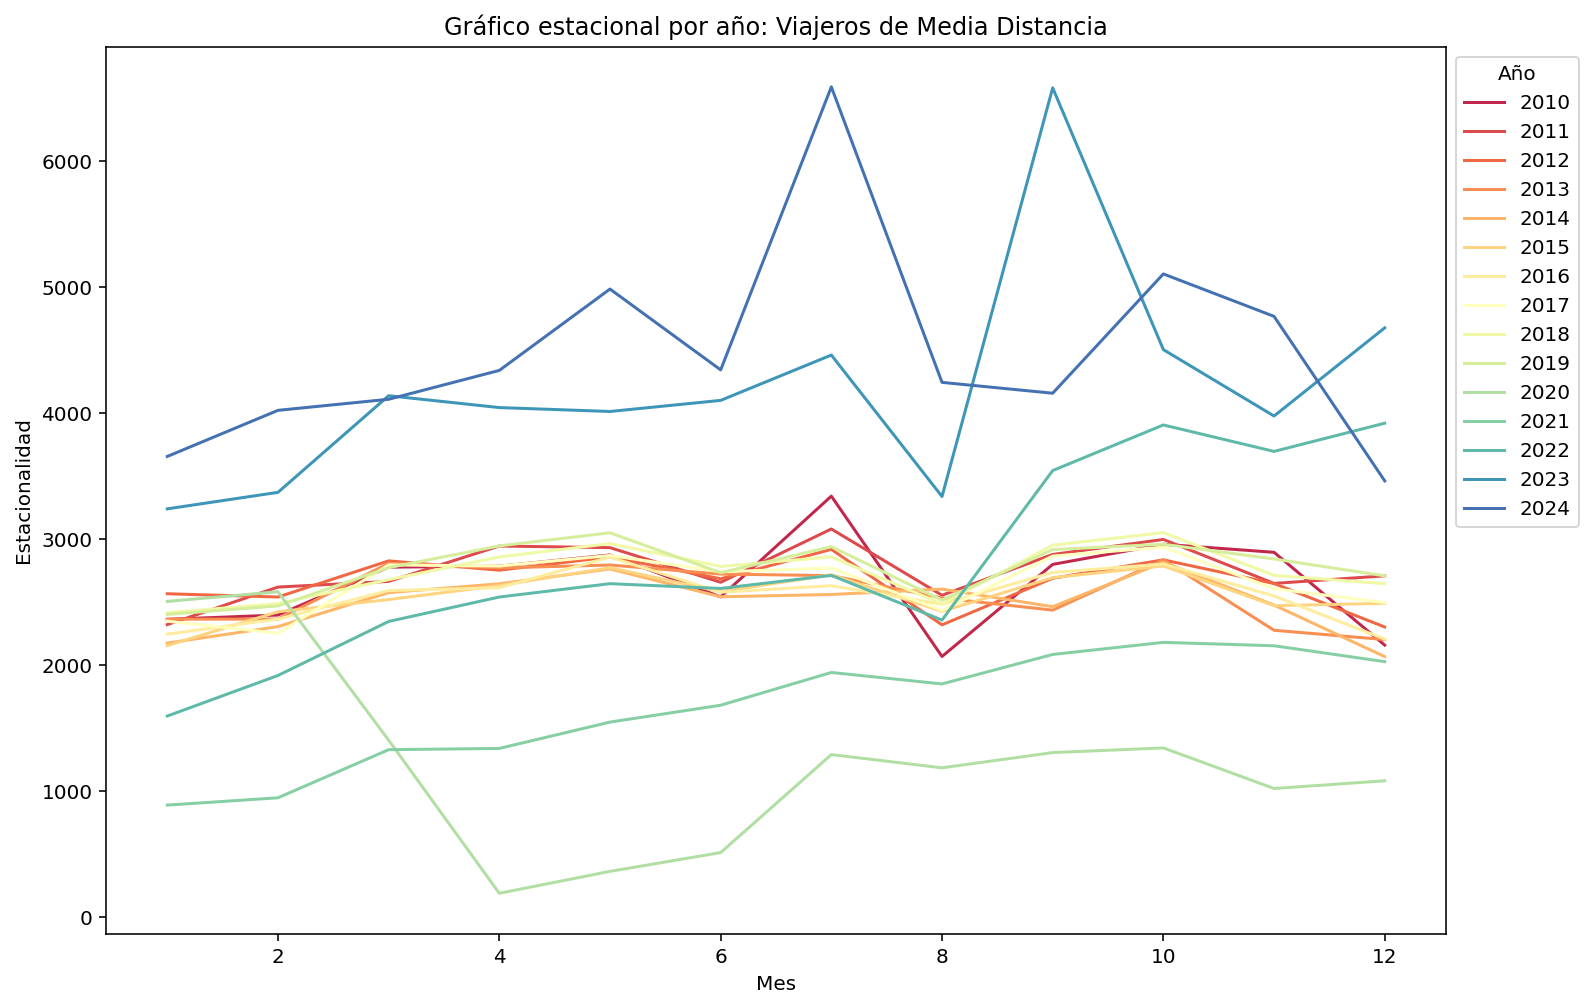
\includegraphics[width=\textwidth]{imgs/seriePorAño.png}
        \caption{} \label{fig:seriePorAño}
    \end{figure}
\end{center}
En la figura \ref{fig:serie}, nos encontramos con una representación tal cual de la serie, dónde se observa una clara estacionalidad en los datos, con valores 
que se repiten en periodos de un año. Además, se observa un brusco descenso en el año 2020, cuadrando con la pandemia, donde el número de viajes se redujo 
bruscamente, hasta llegar casi a 0, debido a las medidas que limitaban la movilidad. En el período post-pandemia, se observa una tendencia claramente al alza, 
que no dura sólo ese año, sino también hasta el presente, a la vez que se observa también una clara estacionalidad, pues si bien los viajeros aumentan cada año
que pasa, se sigue observando un pico en los datos a mediados de año, y un valle hacia finales de año. Esto se ve también en la figura \ref{fig:seriePorAño}, 
donde hemos descompuesto la serie asignando a cada año un color diferente, y hemos representado el número de viajeros en cada mes. Aquí se observa más 
claramente el escaso número de viajeros del año 2020, el ligero aumento que se produjo en 2021, y las cantidades tan elevadas de viajeros que vimos en los dos 
últimos años, así como un claro pico de viajeros que se produce en el mes de julio, seguido de una disminución brusca de los mismos en el mes de agosto, lo 
que se corresponde claramente con el patrón de vacaciones que estamos acostumbrados a ver en España.

\begin{center}
    \begin{figure}[h!]
        \centering
        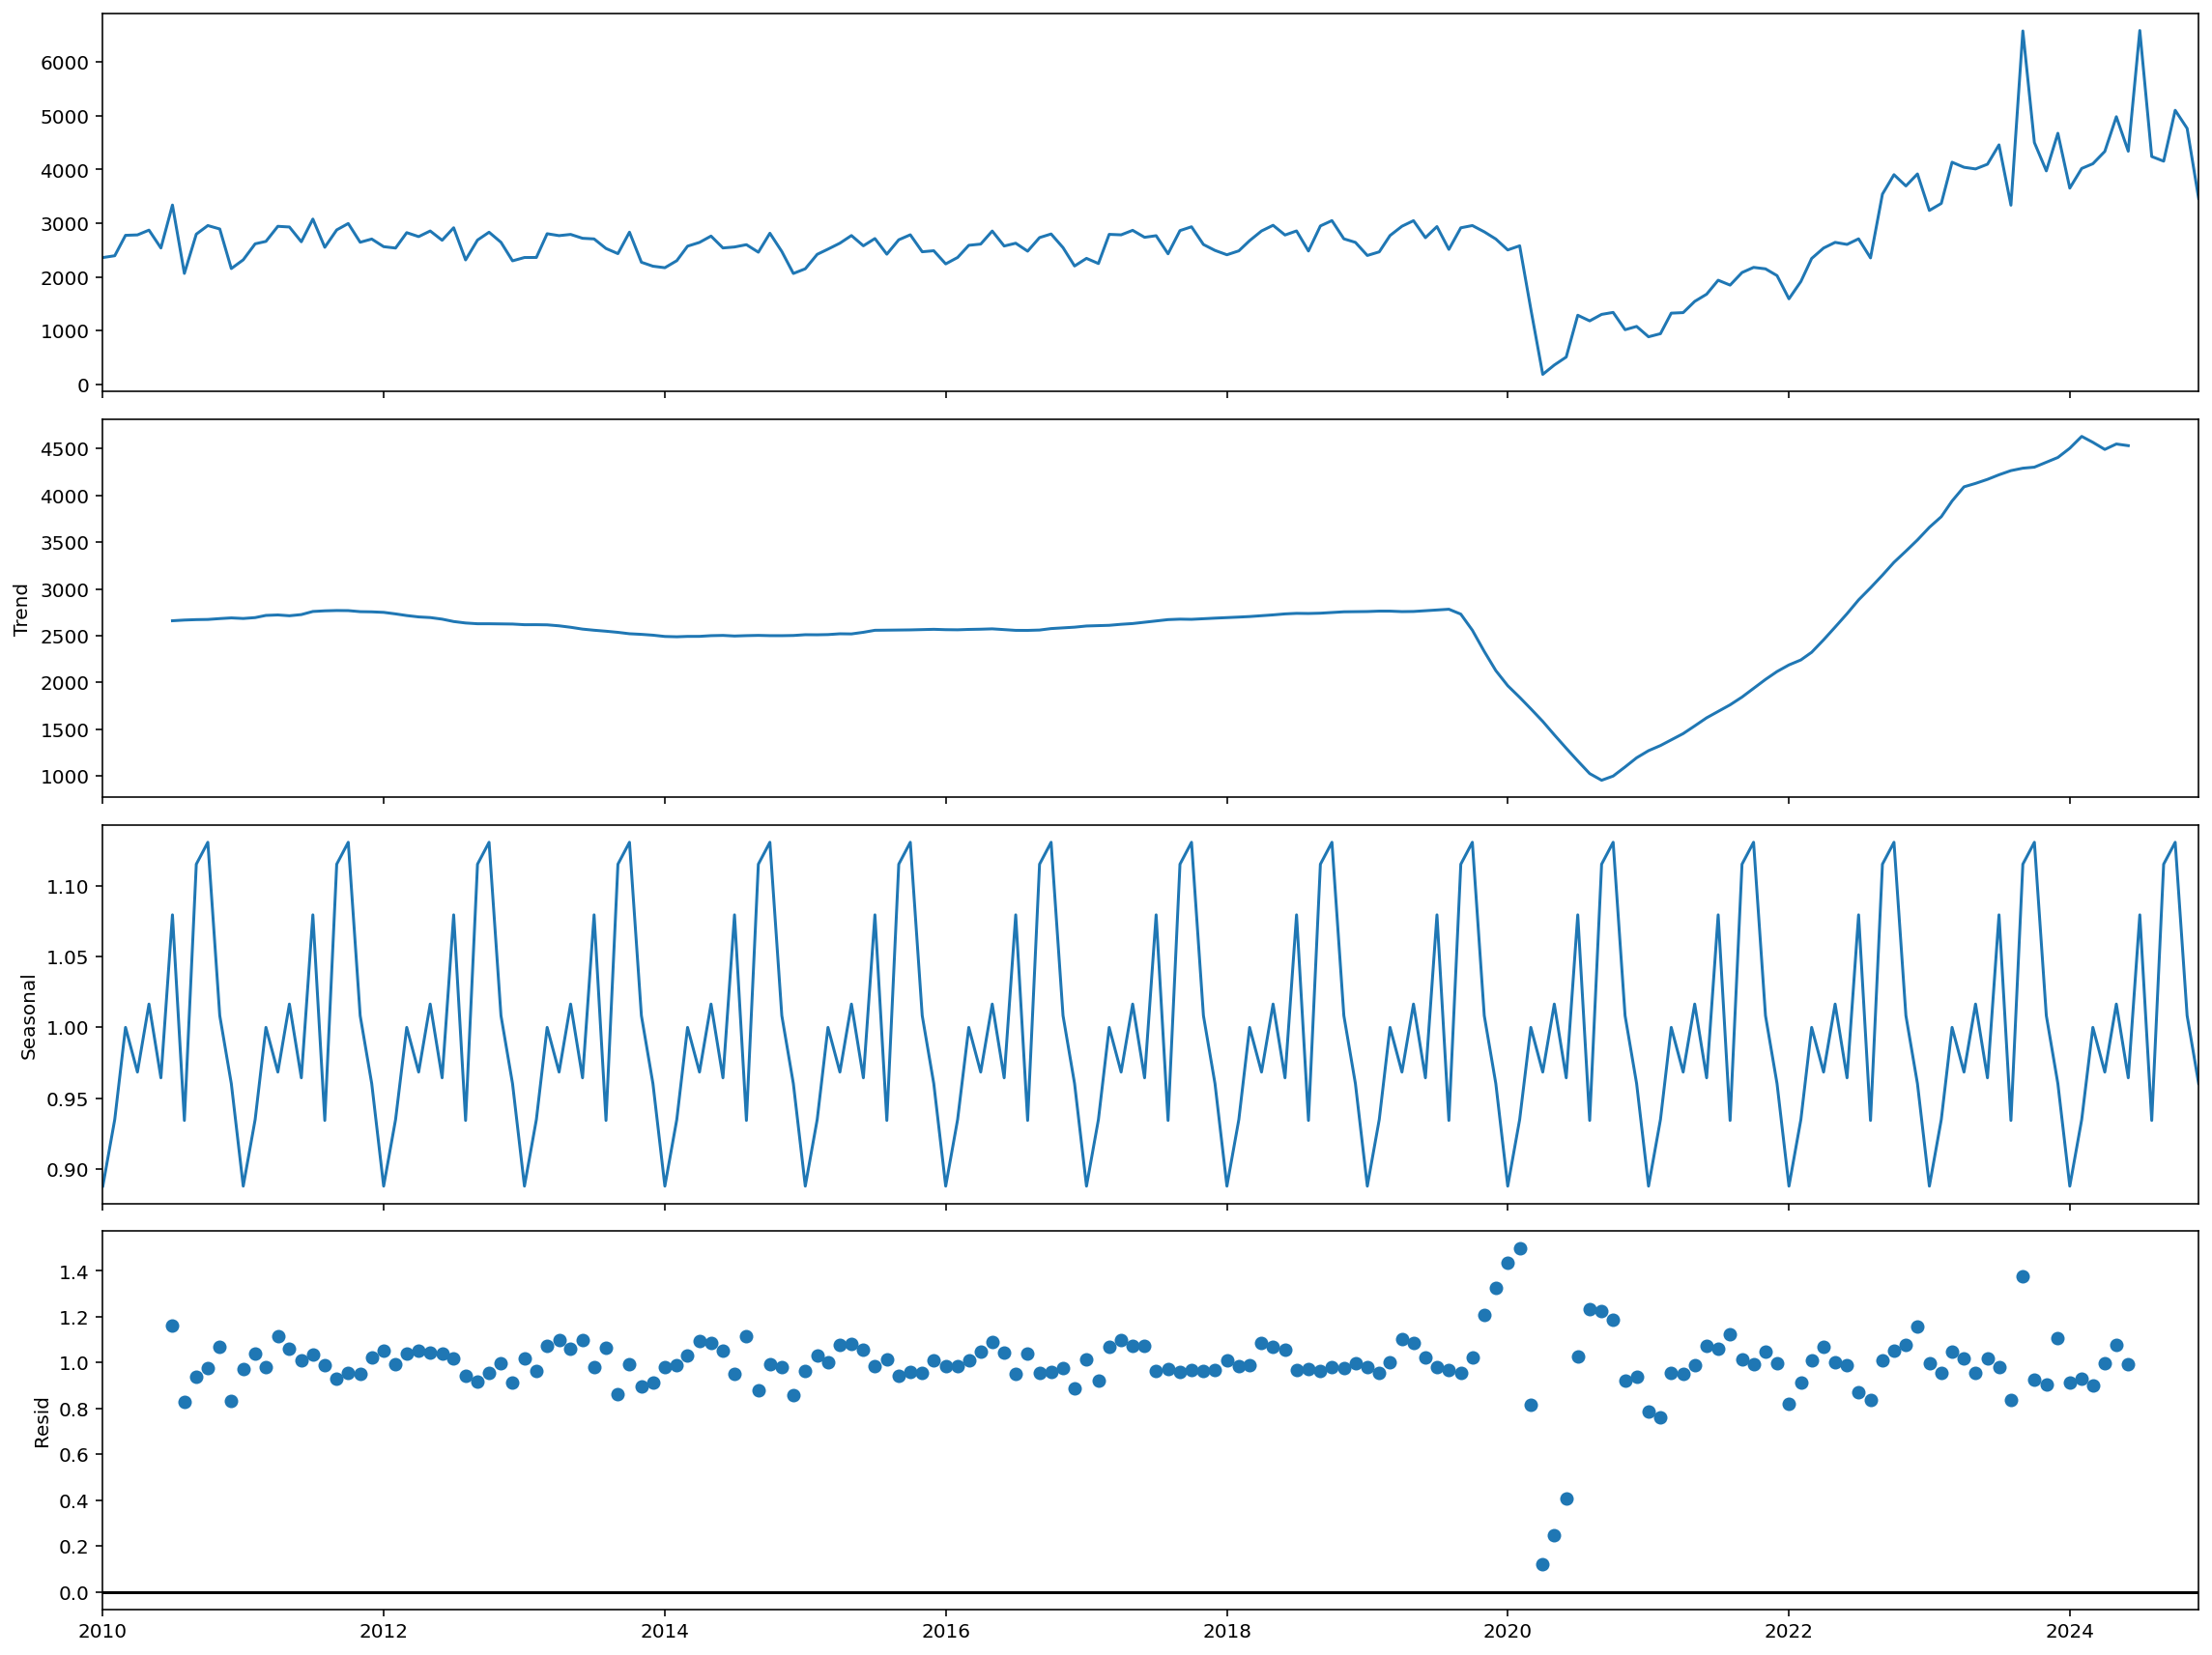
\includegraphics[width=\textwidth]{imgs/descomposicion.png}
        \caption{} \label{fig:descomposicion}
    \end{figure}
\end{center}

Ya que la serie tiene un claro comportamiento estacional, podemos realizar su descomposición estacional, mediante el método \texttt{seasonal\_decompose}. Para 
hacer este método, podemos utilizar un modelo aditivo, en el que los valores desestacionalizados se obtienen sumando las correcciones estacionales a la serie;
o un modelo multiplicativo, donde la serie corregida se obtiene multiplicando la serie original por el componente estacional. Este último será el que usaremos, 
ya que en nuestros datos no tenemos ningún valor que sea 0. Si observamos la gráfica que se produce al realizar esta descomposición, en la figura 
\ref{fig:descomposicion}, vemos que el componente estacional (tercera gráfica) está claramente marcado, lo que quiere decir que la serie tiene un comportamiento 
estacional. Además, este toma valores alrededor de 1, ya que nos indica cuánto aumenta o disminuye el número de viajeros en un mes concreto con respecto a la 
media. En la cuarta gráfica, vemos el componente irregular, mientras que en la tercera observamos la tendencia, donde se ve claramente que la serie tenía una 
tendencia constante hasta que llegó la pandemia, donde se observa un brusco descenso, seguido de una marcada tendencia al alza.

\section{Modelos de suavizado exponencial} \label{suavizado}
En esta sección aplicaremos distintos modelos de suavizado, con el objetivo de determinar finalmente cuál de ellos es mejor. Estos modelos estiman los valores 
de los componentes de la serie en función del tiempo, usando los valores anteriores y suavizándolos empleando coeficientes que minimicen el error producido. 
Crearemos cuatro modelos diferentes partiendo de los datos de train, con el objetivo de realizar diferentes predicciones y compararlas con los datos de test, 
para evaluar que modelo es el que mejor se ajusta.

\subsection{Modelo de suavizado simple} \label{suavizadoSimple}
\begin{center}
    \begin{figure}[h!]
        \centering
        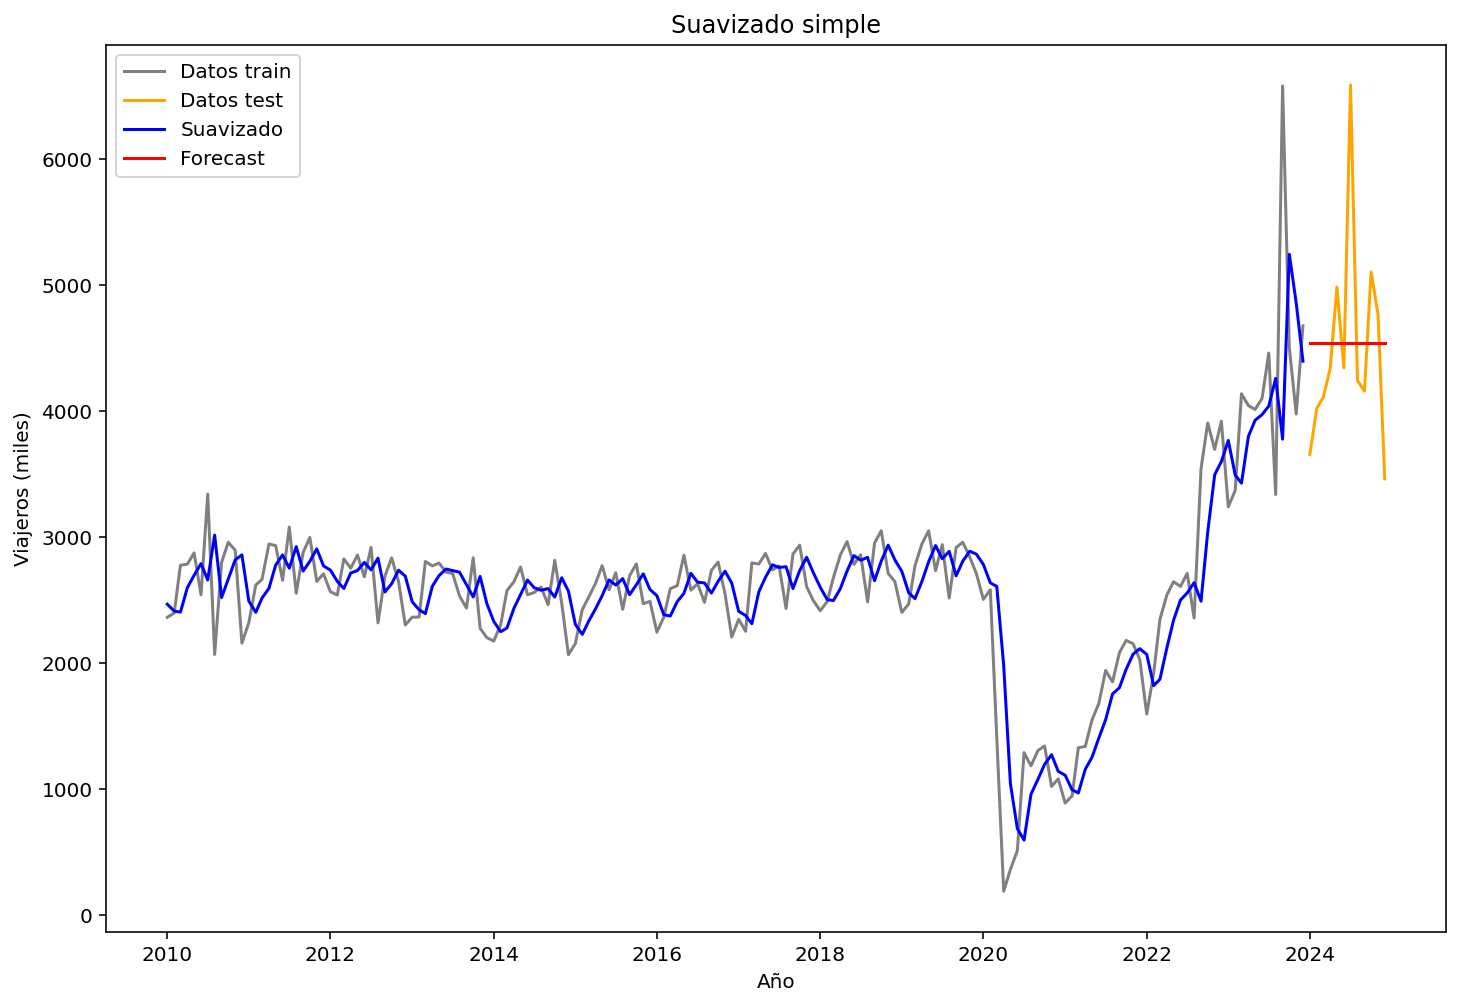
\includegraphics[width=0.75\textwidth]{imgs/suavizadoSimple.png}
        \caption{Modelo de suavizado simple} \label{fig:suavizadoSimple}
    \end{figure}
\end{center}
El modelo de suavizado simple suele usarse cuando la serie no presenta una tendencia relevante, por lo que es casi seguro que podremos desestimarlo de entre 
los modelos candidatos a ser ganadores. Aún así, en la gráfica \ref{fig:suavizadoSimple} se muestra el resultado de la predicción para el último año de este 
modelo, donde se ve que claramente no es correcta, ya que muestra un valor fijo para las predicciones de los 12 meses ya que, como dijimos, este modelo sólo 
se usa para series que no tienen una tendencia muy marcada. Si vemos el parámetro alfa, este es de $0.523406$, mientras que el valor inicial es de $2465.023001$.

\subsection{Modelo de suavizado de Holt} \label{suavizadoHolt}
\begin{center}
    \begin{figure}[h!]
        \centering
        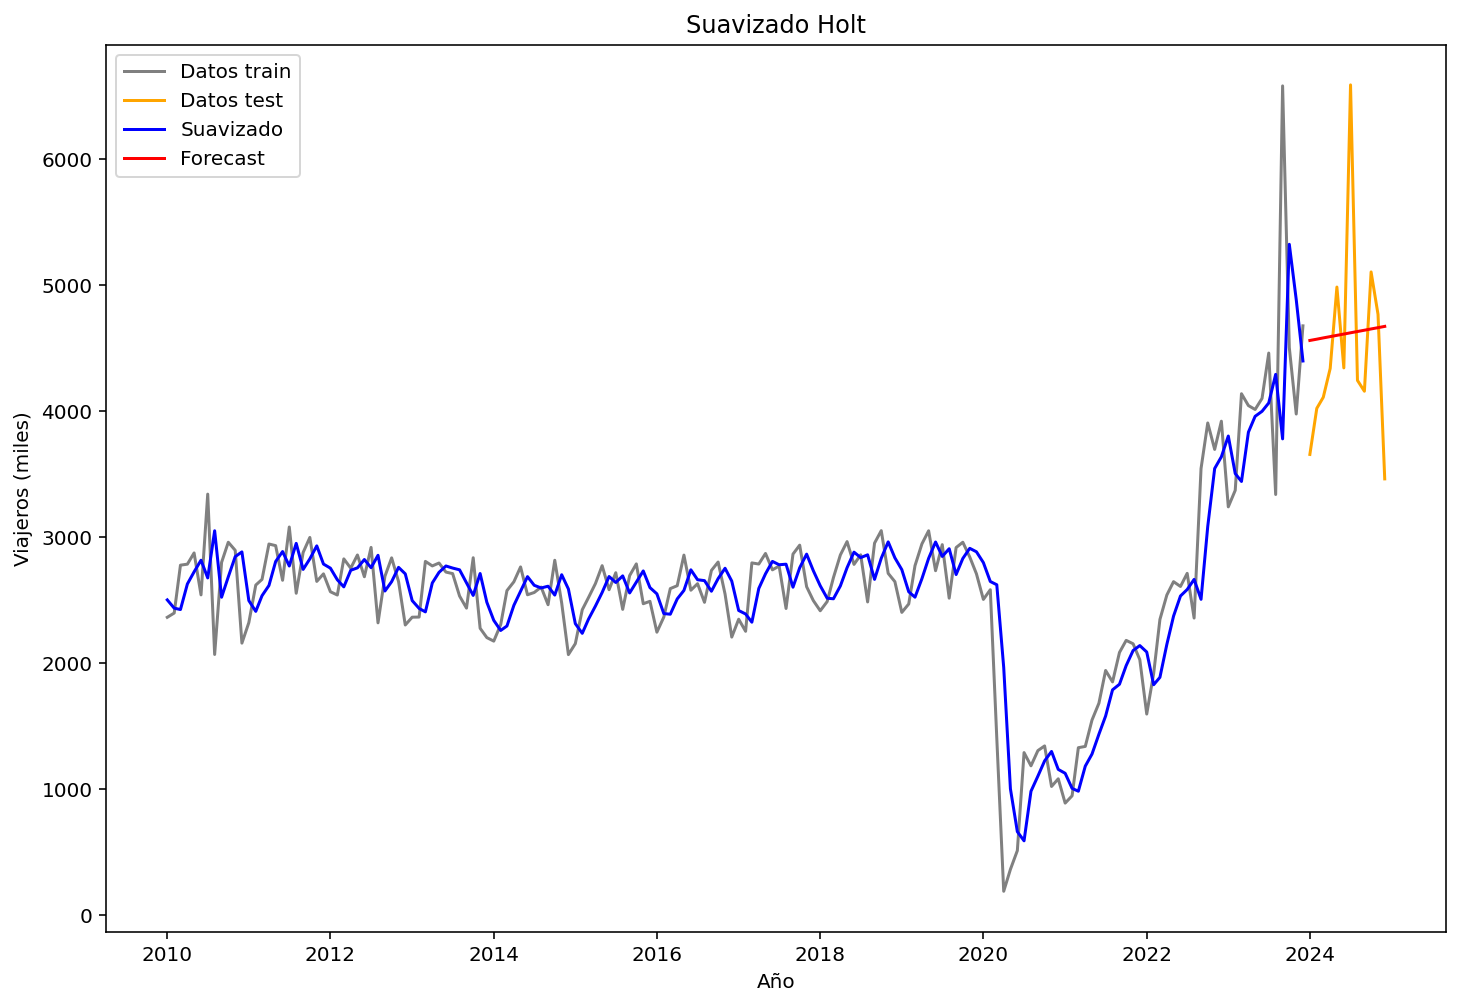
\includegraphics[width=0.75\textwidth]{imgs/suavizadoHolt.png}
        \caption{Modelo de suavizado de Holt} \label{fig:suavizadoHolt}
    \end{figure}
\end{center}
El método de Holt es similar al anterior, pero en este caso presupone que la tendencia es lineal, es decir, que tiene una pendiente variable. De esta forma, 
en este método obtendremos dos parámetros, $\alpha$ y $\beta$, que se corresponden con el factor de suavización del nivel y la tendencia, respectivamente, así 
como el valor inicial de dicho nivel y tendencia. Si aplicamos el modelo y realizamos las predicciones, obtenemos la gráfica de \ref{fig:suavizadoHolt}, donde 
vemos que, aunque las predicciones siguen siendo totalmente erróneas, se aprecia la tendencia creciente que veíamos en los datos. En este caso, los parámetros 
que obtuvimos del modelo son $\alpha=0.547596$, $\beta=0.000100$, $L_{0}=2489.217917$ y $B_{0}=10.117447$.

\subsection{Modelo de tendencia amortiguada} \label{suavizadoAmortiguada}
\begin{center}
    \begin{figure}[h!]
        \centering
        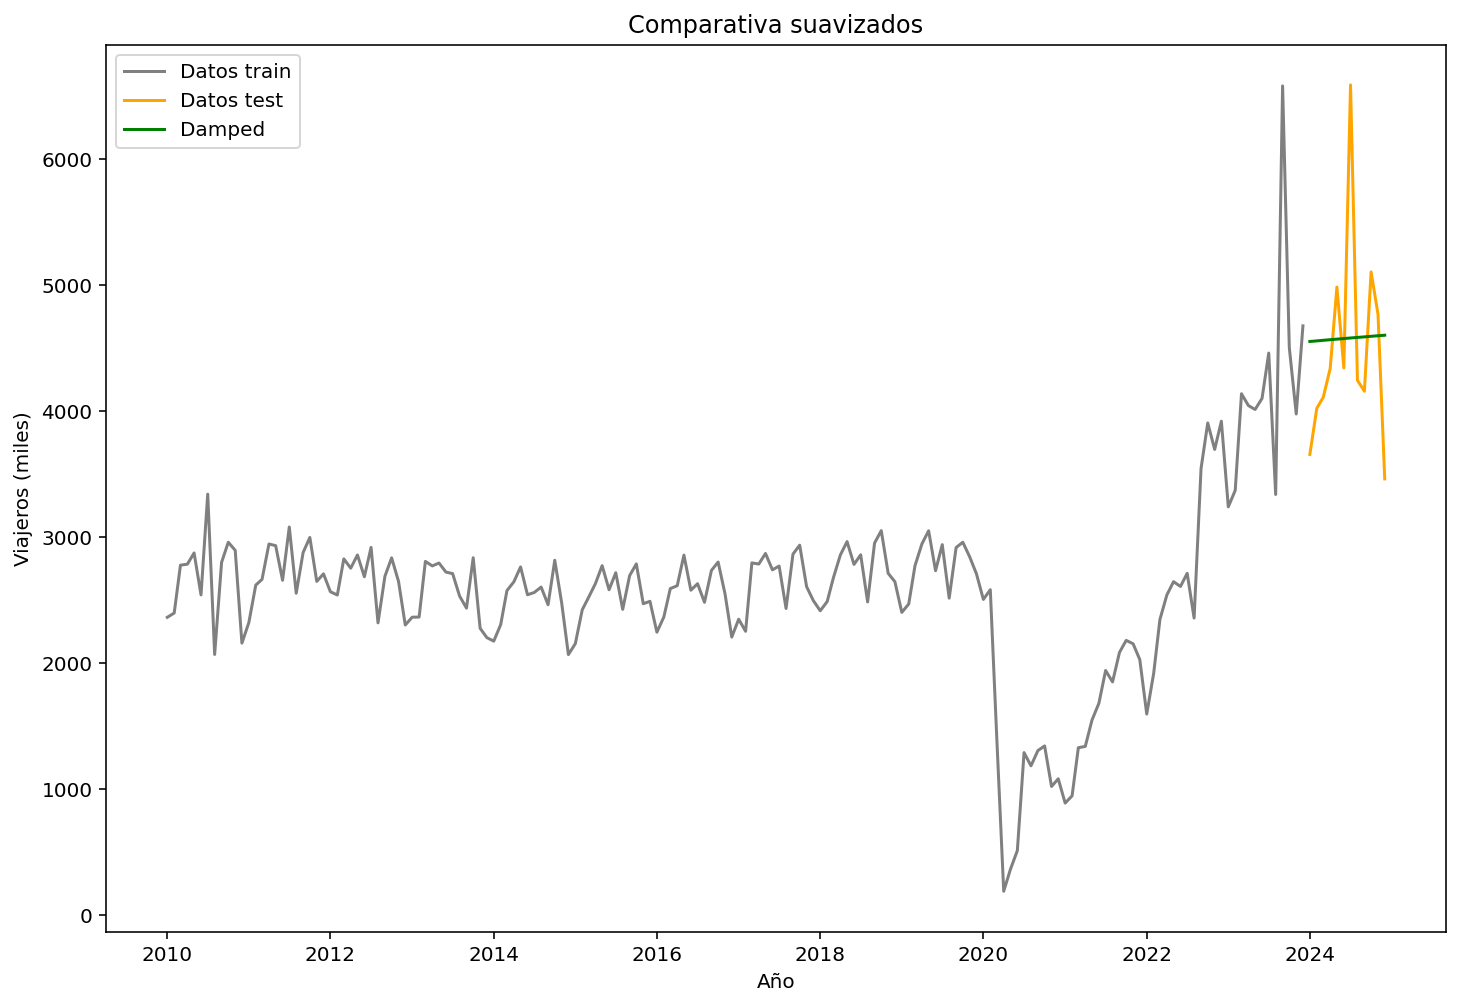
\includegraphics[width=0.75\textwidth]{imgs/suavizadoAmortiguada.png}
        \caption{Modelo de tendencia amortiguada} \label{fig:suavizadoAmortiguada}
    \end{figure}
\end{center}
El modelo o método de tendencia amortiguada es una variación del modelo ed Holt que acabamos de ver en \ref{suavizadoHolt}, que introduce un factor de 
amortiguación para que las predicciones no sean una simple recta, sino que tomen una forma ajustada más a una curva. Esto vendrá dado por el parámetro $\phi$ 
del modelo, que devuelve además los dos factores anteriores, así como los valores iniciales. Podemos ver las predicciones que ha realizado en la figura 
\ref{fig:suavizadoAmortiguada}. De esta forma, tenemos un $\alpha=0.521807$ y un $\beta=0.001862$, muy similares a los parámetros del anterior modelo, con un 
$L_{0}=2488.744544$ y $B_{0}=8.973355$, también similares a los anteriores. Sin embargo, si analizamos el $\phi$, vemos que es $\phi=0.990017$, prácticamente
1, lo cual indica que no tiene apenas efecto. Es decir, que el modelo de tendencia amortiguada nos producirá los mismos resultados casi que el modelo de Holt.
Esto podemos verlo fácilmente en la figura \ref{fig:suavizadoComp3}, donde comparamos las predicciones del modelo de suavizado simple, el de Holt y este de la 
tendencia amortiguada. En él, vemos en rojo las predicciones del modelo simple, que eran una simple línea sin pendiente, y tenemos en azul las predicciones 
del método de Holt, y en verde las del método de tendencias amortiguadas, donde vemos que ambas toman unos valores bastantes similares, estando la pendiente 
de este último modelo un poco menos pronunciada que la del anterior.
\begin{center}
    \begin{figure}[h!]
        \centering
        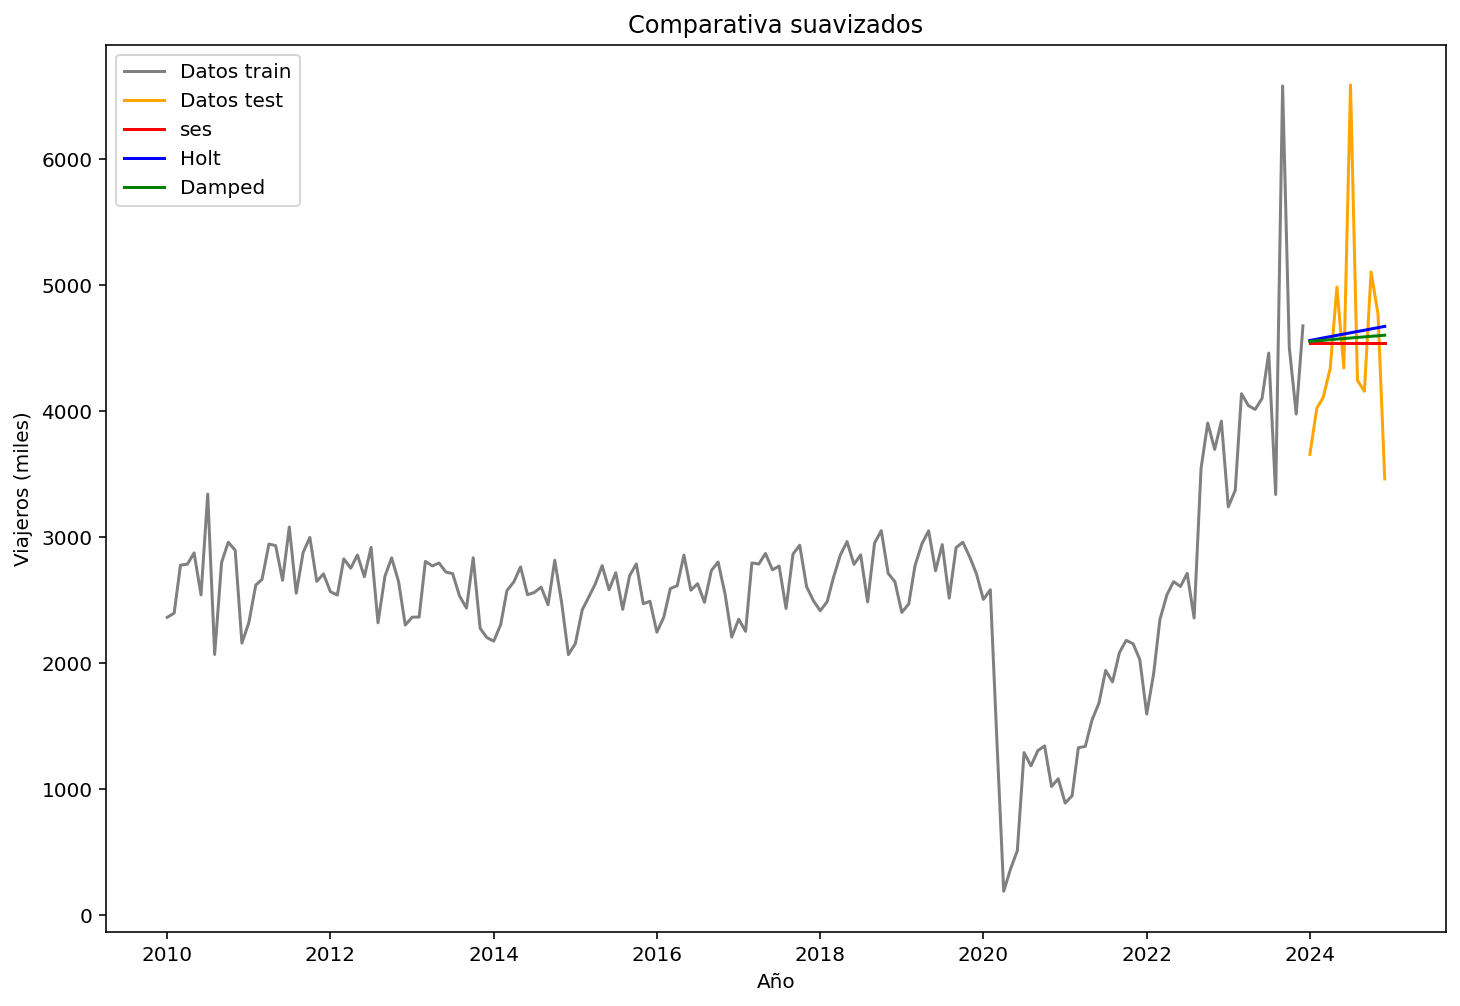
\includegraphics[width=0.75\textwidth]{imgs/suavizadoComp3.png}
        \caption{Comparación: suavizado simple, Holt y \textit{damped}} \label{fig:suavizadoComp3}
    \end{figure}
\end{center}

\subsection{Modelo de suavizado de Holt-Winters} \label{suavizadoHoltWinters}
\begin{center}
    \begin{figure}[h!]
        \centering
        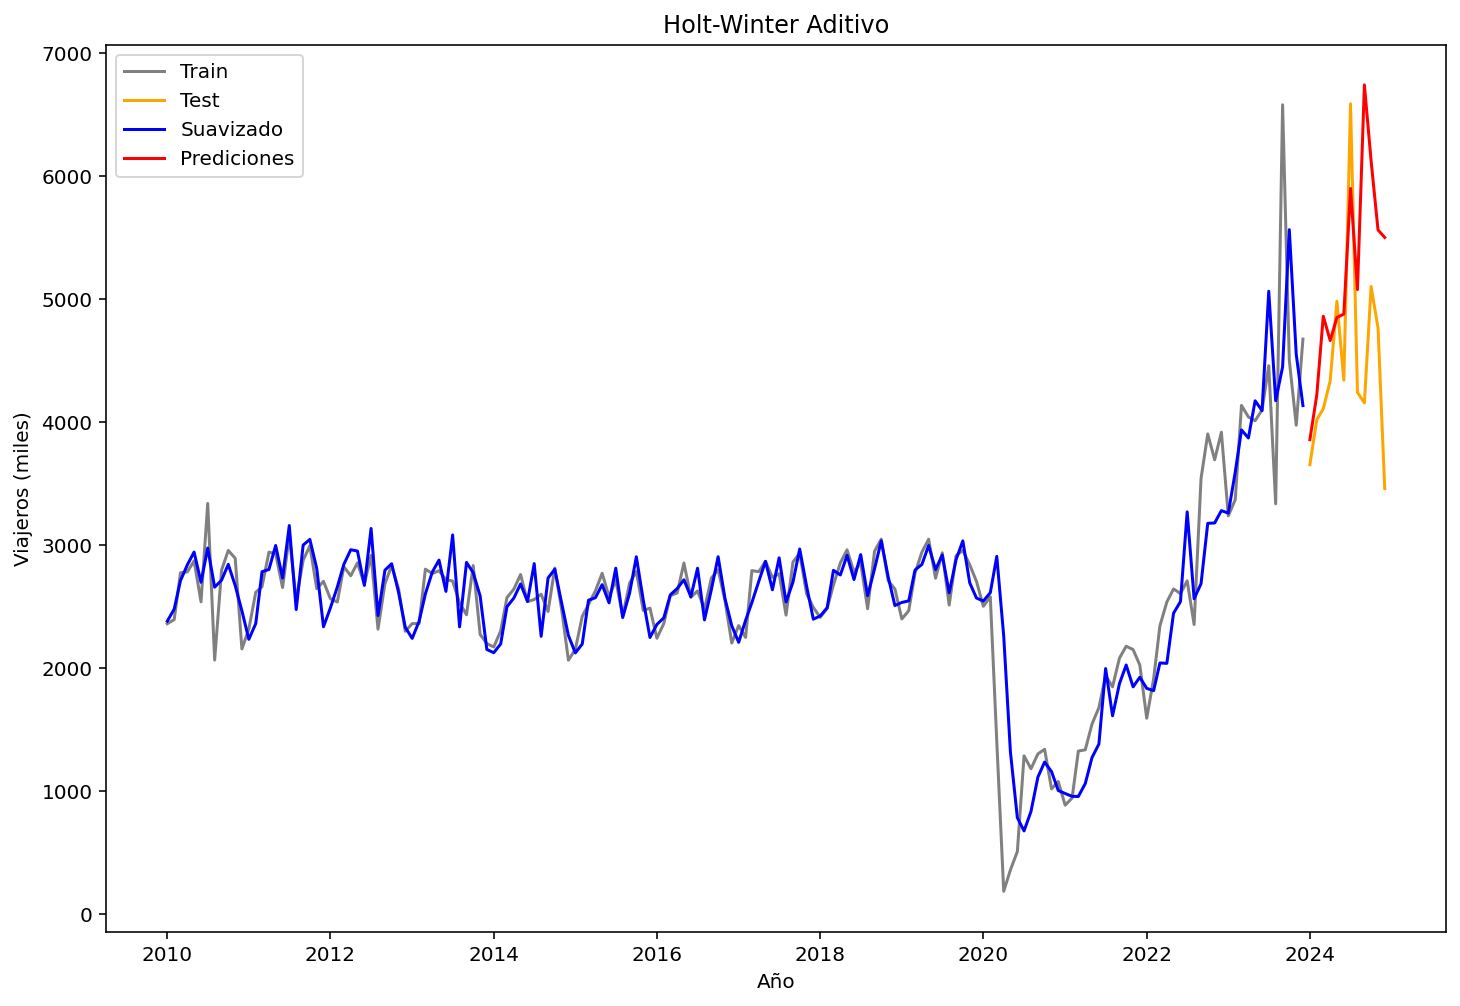
\includegraphics[width=0.75\textwidth]{imgs/suavizadoHoltWinters.png}
        \caption{Modelo de tendencia amortiguada} \label{fig:suavizadoHoltWinters}
    \end{figure}
\end{center}
Por último, aplicaremos el modelo de suavizado de Holt-Winters, un modelo que a priori debería ser más adecuado, ya que incorpora la estacionalidad mediante un
coeficiente que multiplica a la tendencia. Los valores iniciales de la tendencia son estimados a partir de la media de los valores del primer ciclo; la pendiente 
se estima a partir de las diferencias en dos ciclos completos; y los índices estacionales, con los valores del primer periodo. En este caos, tenemos como 
parámetros los que se ven en la tabla \ref{tab:paramsHoltW}. Tenemos los parámetros de antes ($\alpha, \beta, L_{0} y B_{0}$), a los que se suma $\gamma$, que 
representa cuánto afecta la información nueva al patrón estacional; y los distintos parámetros iniciales de los factores estacionales $S_{0}$ a $S_{11}$, que,
ya que empleamos un modelo multiplicativo, nos indica cuánto se desvía ese mes en concreto de la media, ya sea con más viajeros (mayor que 1) o menos viajeros.
\begin{table}[]
    \begin{center}
        \begin{tabular}{|c|c|c|}
            \hline
            \textbf{Parámetro} & \textbf{Abreviatura} & \textbf{Valor} \\
            \hline
            smoothing\_level    & $\alpha$ & 0.464643 \\
            smoothing\_trend    & $\beta$ & 0.0244549 \\
            smoothing\_seasonal & $\gamma$ & 0.178452 \\
            initial\_level      & $L_{0}$ & 2650.66 \\
            initial\_trend      & $B_{0}$ & 1.00441 \\
            initial\_seasons.0  & $S_{0}$ & 0.894502 \\
            initial\_seasons.1  & $S_{1}$ & 0.931432 \\
            initial\_seasons.2  & $S_{2}$ & 1.03039 \\
            initial\_seasons.3  & $S_{3}$ & 1.06354 \\
            initial\_seasons.4  & $S_{4}$ & 1.10814 \\
            initial\_seasons.5  & $S_{5}$ & 1.02364 \\
            initial\_seasons.6  & $S_{6}$ & 1.15761 \\
            initial\_seasons.7  & $S_{7}$ & 0.974111 \\
            initial\_seasons.8  & $S_{8}$ & 1.1079 \\
            initial\_seasons.9  & $S_{9}$ & 1.1417 \\
            initial\_seasons.10 & $S_{10}$ & 1.05023 \\
            initial\_seasons.11 & $S_{11}$ & 0.930051 \\
            \hline
        \end{tabular}
        \caption{Parámetros del modelo de Holt-Winters}
        \label{tab:paramsHoltW}
    \end{center}
\end{table}

Está claro que este es el modelo de suavizado más adecuado, ya que, como se ve en la figura \ref{fig:suavizadoHoltWinters}, las predicciones se ajustan casi 
perfectamente con los datos que teníamos de test, sólo se observa que, para los últimos meses de 2024, no percibe a la perfección la disminución de viajeros
del mes de septiembre, y obtiene unos valores más elevados. 

En la tabla \ref{tab:prediccionesHoltWinter}, podemos ver, por una parte, la predicción que ha 
realizado este modelo y por otro, los resultados que teníamos reservados de los datos de test. Vemos que las diferencias, salvo en estos últimos meses que 
comentamos, donde son de 2500 miles de viajeros que ha estimado de más en el mes de septiembre, o 2000 miles de viajeros de más en diciembre, en el resto de 
meses la estimación se ajusta bastante a la realidad.

Como es evidente, no va a ser una predicción exacta, ni mucho menos, porque tampoco es lo que busca 
este método, pero sí que se corresponde de una forma bastante fiel a los datos que se han observado, teniendo en cuenta también que los datos presentan una 
tendencia creciente que es siempre más difícil de predecir. 
\begin{table}[h!]
    \begin{center}
        \begin{tabular}{|c|c|c|}
            \hline
            \textbf{Mes} & \textbf{Predicción} & \textbf{Datos test} \\
            \hline
            Enero 2024         & 3857.368419 & 3654 \\
            Febrero 2024       & 4220.702156 & 4020 \\
            Marzo 2024         & 4860.868766 & 4108 \\
            Abril 2024         & 4663.238474 & 4337 \\
            Mayo 2024          & 4850.431828 & 4983 \\
            Junio 2024         & 4878.574812 & 4341 \\
            Julio 2024         & 5899.436039 & 6588 \\
            Agosto 2024        & 5077.671698 & 4242 \\
            Septiembre 2024    & 6741.756478 & 4156 \\
            Octubre 2024       & 6124.685444 & 5103 \\
            Noviembre 2024     & 5562.474281 & 4766 \\
            Diciembre 2024     & 5501.244563 & 3460 \\
            \hline
        \end{tabular}
        \caption{Predicciones del modelo de Holt-Winters}
        \label{tab:prediccionesHoltWinter}
    \end{center}
\end{table}

\section{Modelos ARIMA}
En esta sección crearemos, por una parte, un modelo ARIMA de forma manual, ajustando los parámetros en base a lo observado en los correlogramas; y por otra 
parte, un modelo ARIMA de forma automática, empleando las funciones proporcionadas en Python.

\newpage

\appendix
\section{Anexo: Código de la práctica}\label{anexo1}
\lstinputlisting[language=Python]{codigoMineria3.py}
\end{sloppypar}
\end{document}
